\documentclass[12pt]{article}
\usepackage{array}
\usepackage{amsmath}
\usepackage{mathtools}
\usepackage{gensymb}
\usepackage{graphicx}
\usepackage{float}
\usepackage{caption}

\allowdisplaybreaks

\def\E{\mathcal{E}}

\begin{document}
    \title{The Electromotive Force and Internal Resistance of a Battery}
    \author{Ryan Coyne}
    \maketitle
    \section*{Abstract/Procedure/Conclusion}
        In this lab, we measured the electromotive force, \(\E\), and internal resistance, \(r\) of a battery using resistors in a circuit with the battery and an ammeter. We used a circuit with resistors in series and a circuit with resistors in parallel.  When measuring using the series circuit, \(\E\) was \((1.544 \pm 0.023)\) V and \(r\) was \((8.54 \pm 0.29)\ \Omega\). When measuring using the parallel circuit, \(\E\) was \((0.9238 \pm 0.0045)\) V and \(r\) was \((1.21 \pm 0.020)\ \Omega\). The values for \(\E\) and \(r\) in each circuit were very different, likely because the battery's internal resistance depends on the current flowing through it. 

        To calculate these values, we use Ohm's law, Kirchhoff's loop law, and Kirchhoff's junction law. Ohm's law is 
        \begin{equation*}
            V=IR
        \end{equation*}
        where \(V\) is the voltage drop over a resistor, \(I\) is the current through the resistor, and \(R\) is the resistance of the resistor. Kirchhoff's loop law says that the voltage drop around any loop in the circuit is zero in total. Kirchhoff's junction law says that the total current entering a junction is equal to the total current exiting the junction.
        \begin{figure}[H]
            \centering
            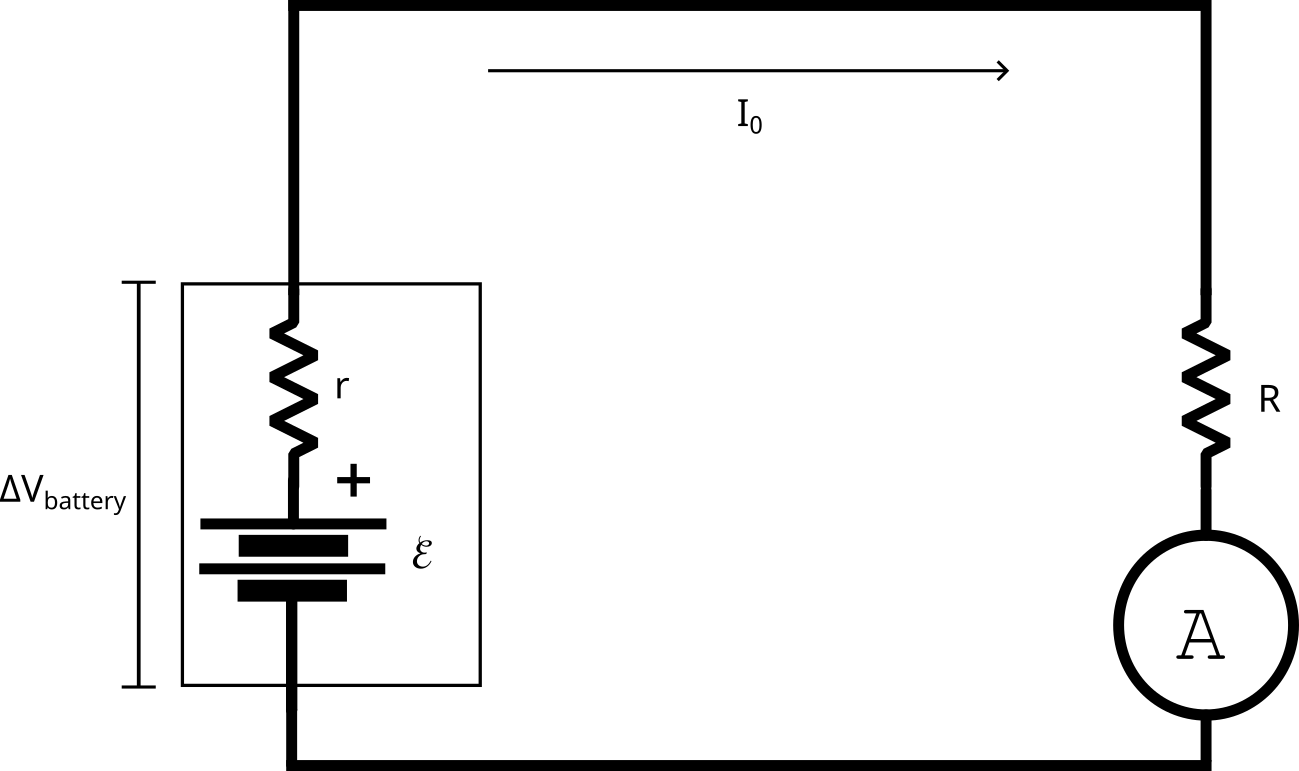
\includegraphics[width=0.75\linewidth]{fig1.png}
            \caption{Initial circuit}
        \end{figure}
        \begin{figure}[H]
            \centering
            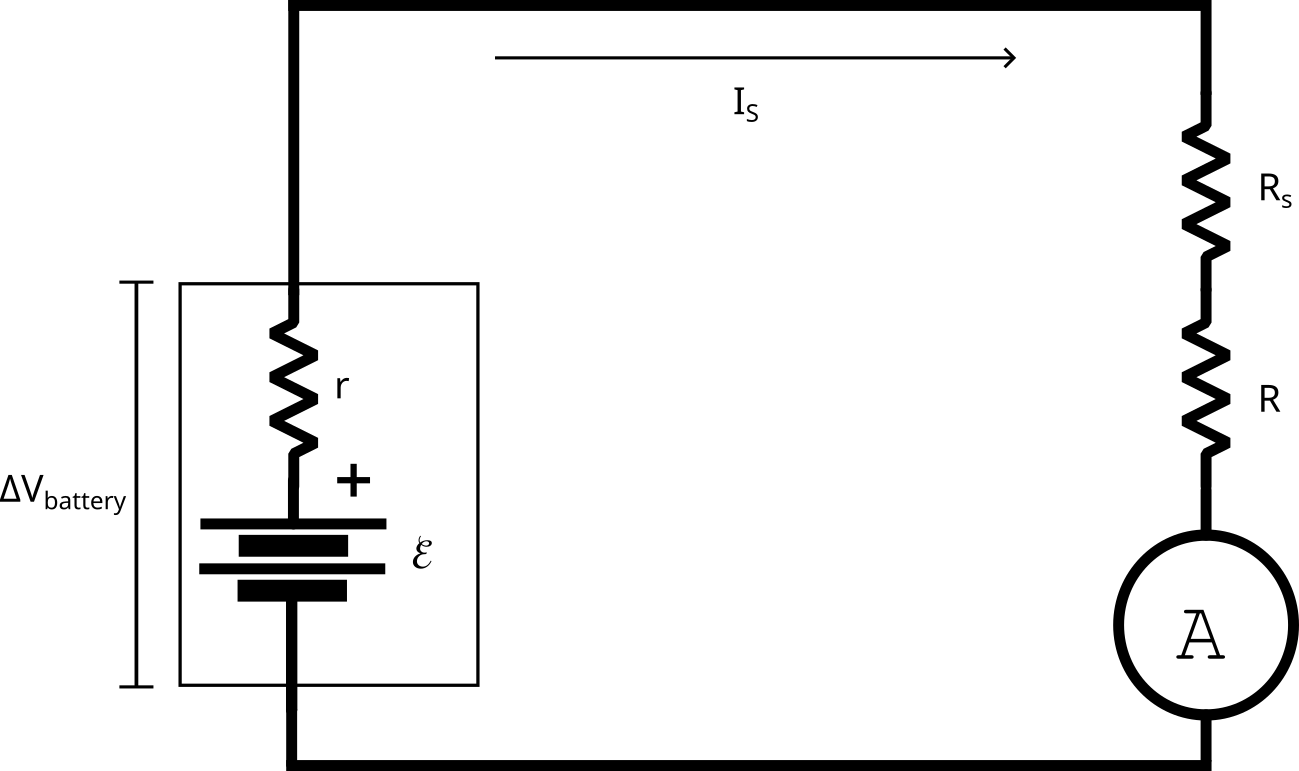
\includegraphics[width=0.75\linewidth]{fig2.png}
            \caption{Resistors in series}
        \end{figure}
        \begin{figure}[H]
            \centering
            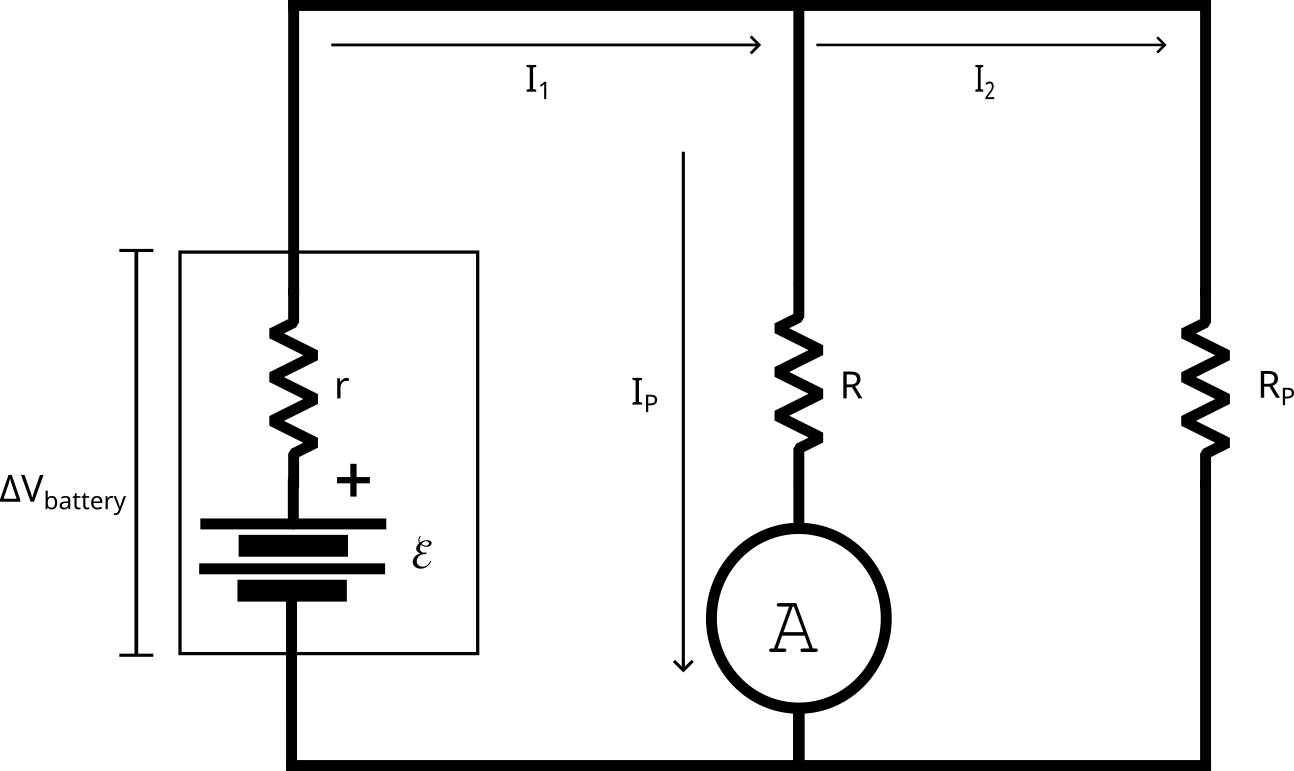
\includegraphics[width=0.75\linewidth]{fig3.png}
            \caption{Resistors in parallel}
        \end{figure}
    \section*{Data}
        \begin{figure}[H]
            \centering
            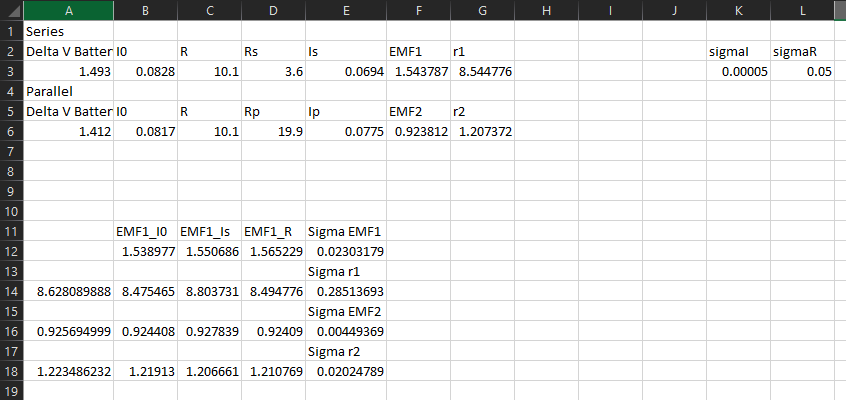
\includegraphics[width=0.85\linewidth]{data.png}
        \end{figure}
    \section*{Calculations}
    \begin{alignat*}{3}
        &(1)~~&&\E - I_0r - I_0R = 0\\
        &(2)~~&&\E - I_sr-I_sR-I_sR_s=0\\
        &(2)-(1)~~&&-I_sr+I_0r+I_0R-I_sR-I_sR_s=0\\
        &&&r(I_s+I_0)=I_s(R_s+R)-I_0R\\
        &&&r=\frac{I_s(R_s+R)-I_0R}{I_s+I_0}\\
        &&&r=\frac{\E-I_0R}{I_0}\\
        &&&\E-I_s\frac{\E-I_0R}{I_0}-I_sR-I_sR_s = 0\\
        &&&\E(1-\frac{I_s}{I_0})=I_sR_s\\
        &&&\E=\frac{I_sR_s}{1-\frac{I_s}{I_0}}\\
        &&&\E=\frac{I_0I_sR_s}{I_0-I_s}
    \end{alignat*}
\end{document}